%% This is the ctufit-thesis example file. It is used to produce theses
%% for submission to the Czech Technical University, Faculty of Information Technology.
%%
%% This is version 1.8.1, built 27. 10. 2026.
%% 
%% Get the newest version from
%% https://gitlab.fit.cvut.cz/theses-templates/FITthesis-LaTeX
%%
%%
%% Copyright 2024, Tomas Novacek
%% Copyright 2021, Eliska Sestakova and Ondrej Guth
%%
%% This work may be distributed and/or modified under the
%% conditions of the LaTeX Project Public License, either version 1.3
%% of this license or (at your option) any later version.
%% The latest version of this license is in
%%  https://www.latex-project.org/lppl.txt
%% and version 1.3 or later is part of all distributions of LaTeX
%% version 2005/12/01 or later.
%%
%% This work has the LPPL maintenance status `maintained'.
%%
%% The current maintainer of this work is Tomas Novacek (novacto3@fit.cvut.cz).
%% Alternatively, submit bug reports to the tracker at
%% https://gitlab.fit.cvut.cz/theses-templates/FITthesis-LaTeX/issues
%%
%%

% Build: latexmk -xelatex ctufit-thesis.tex (XeLaTeX + biber; also works on Overleaf with XeLaTeX)
% arara: xelatex
% arara: biber
% arara: xelatex
% arara: xelatex

%%%%%%%%%%%%%%%%%%%%%%%%%%%%%%%%%%%%%%%%%
% CLASS OPTIONS
% language: czech/english/slovak
% thesis type: bachelor/master/dissertation/doctoral-report
% electronic (oneside) or printed (twoside), twoside is default
% paragraph - if passed, this optional argument sets paragraphs as the deepest level of headers, styles it, numbers it and adds it to the Table of Contents. Use with care! Normally, it is considered unwise to use it, since it is too deep.
% colour: bw for black&white OR no option for default colour scheme
%%%%%%%%%%%%%%%%%%%%%%%%%%%%%%%%%%%%%%%%%
\documentclass[czech,bachelor,oneside]{ctufit-thesis}

%%%%%%%%%%%%%%%%%%%%%%%%%%%%%%%%%%
% FILL IN THIS INFORMATION
%%%%%%%%%%%%%%%%%%%%%%%%%%%%%%%%%%
\ctufittitle{Automatické plánování s~numerickými doménami pro strategickou hru StarCraft~II} % replace with the title of your thesis
\ctufitauthorfull{Daria Krylova} % replace with your full name (first name(s) and then family name(s) / surname(s)) including academic degrees
\ctufitauthorsurnames{Krylova} % replace with your surname(s) / family name(s)
\ctufitauthorgivennames{Daria} % replace with your first name(s) / given name(s)
\ctufitsupervisor{prof.\,RNDr.\,Pavel Surynek,\,Ph.D.} % replace with name of your supervisor/advisor (include academic degrees)
\ctufitdepartment{Katedra aplikované matematiky} % replace with the department of your defence
\ctufitprogram{Informatika} % replace with your study program
\ctufitspecialisation{Umělá inteligence 2021} % replace with your specialisation
\ctufityear{2026} % replace with the year of your defence
\ctufitdeclarationplace{Praze} % replace with the place where you sign the declaration
\ctufitdeclarationdate{\today} % replace with the date of signature of the declaration
\ctufitabstractCZE{TODO: abstrakt (T6.5).}
\ctufitabstractENG{TODO: abstract (T6.5).}
\ctufitkeywordsCZE{StarCraft II, automatické plánování, numerické domény, PDDL, ENHSP, RTS hry}
\ctufitkeywordsENG{StarCraft II, automated planning, numeric domains, PDDL, ENHSP, RTS games}
%%%%%%%%%%%%%%%%%%%%%%%%%%%%%%%%%%
% END FILL IN
%%%%%%%%%%%%%%%%%%%%%%%%%%%%%%%%%%

%%%%%%%%%%%%%%%%%%%%%%%%%%%%%%%%%%
% CUSTOMISATION of this template
% Skip this part or alter it if you know what you are doing.
%%%%%%%%%%%%%%%%%%%%%%%%%%%%%%%%%%

% hyperlinks
\hypersetup{
    pdfpagelayout=TwoPageRight,
    colorlinks=false,
    allcolors=decoration,
    pdfborder={0 0 0.1}
}

% uncomment the following to hide all hyperlinks
%\hypersetup{hidelinks}

% uncomment the following to change the colour of all hyperlinks to CTU blue
%\hypersetup{allbordercolors=decoration}


%%%%%%%%%%%%%%%%%%%%%%%%%%%%%%%%%%
% CUSTOMIZATION of this template END
%%%%%%%%%%%%%%%%%%%%%%%%%%%%%%%%%%


%%%%%%%%%%%%%%%%%%%%%%
% PACKAGES SETTINGS
% You may choose to modify this part.
%%%%%%%%%%%%%%%%%%%%%%
\usepackage[style=iso-numeric,backend=biber]{biblatex}
\addbibresource{text/bib-database.bib}

\usepackage{dirtree}
\usepackage{lipsum,tikz}
% babel: Czech makes "-" active, which breaks TikZ coordinates and arrows otherwise
\usetikzlibrary{babel,positioning,arrows.meta,calc}
\usepackage{xurl}
\usepackage{listings}
\usepackage{algorithm2e}

\usepackage{graphicx}
\usepackage{subcaption}

\usepackage{booktabs}
\usepackage{array}
\usepackage{tabularx}
\setlength{\emergencystretch}{3em} % long identifiers in Czech text, also in the front matter
\graphicspath{{figures/}{images/}} % figures/ is generated by experiments/plots.py
%%%%%%%%%%%%%%%%%%%%%%
% PACKAGES SETTINGS END
%%%%%%%%%%%%%%%%%%%%%%

\begin{document}
\frontmatter\frontmatterinit % do not remove these two commands

\thispagestyle{empty}\maketitle % do not remove these two commands

\ctufitincludeassignment[pages={1-}]{assignment.pdf} % replace this file with your thesis assignment generated from ProjectsFIT. Remove for doctoral report and dissertation thesis. For bachelor's and master's theses, the assignment is mandatory.

\imprintpage % do not remove this command
\stopTOCentries

%%%%%%%%%%%%%%%%%%%
% ACKNOWLEDGMENT
% FILL IN / MODIFY
% This is a place to thank people for helping you. It is common to thank your supervisor.
%%%%%%%%%%%%%%%%%%%
\begin{acknowledgmentpage}
	Tímto bych ráda poděkovala svému vedoucímu práce, prof.~RNDr.~Pavlu Surynkovi,~Ph.D., za odborné vedení této práce.
\end{acknowledgmentpage}
%%%%%%%%%%%%%%%%%%%
% ACKNOWLEDGMENT END
%%%%%%%%%%%%%%%%%%%


%%%%%%%%%%%%%%%%%%%
% DECLARATION
% FILL IN / MODIFY
%%%%%%%%%%%%%%%%%%%
% INSTRUCTIONS
% ENG: Choose one of the approved texts of the declaration. DO NOT CREATE YOUR OWN. Select one of the approved texts according to https://courses.fit.cvut.cz/SFE/license.html (Licensing of Final Theses)
% CZE/SLO: Vyberte jedno z fakultou schválených prohlášení. NEVKLÁDEJTE VLASTNÍ TEXT. Vyberte jedno ze schválených prohlášení podle https://courses.fit.cvut.cz/SZZ/prace/licence.html (Licence k závěrečným pracem)
\begin{declarationpage}
	Prohlašuji, že jsem předloženou práci vypracovala samostatně a~že jsem uvedla veškeré
	použité informační zdroje v~souladu s~Metodickým pokynem o~dodržování etických
	principů při přípravě vysokoškolských závěrečných prací.
	
	Beru na vědomí, že se na moji práci vztahují práva a povinnosti vyplývající ze zákona
	č.~121/2000~Sb., autorského zákona, ve znění pozdějších předpisů, zejména
	skutečnost, že České vysoké učení technické v~Praze má právo na uzavření licenční
	smlouvy o~užití této práce jako školního díla podle §~60~odst.~1~citovaného zákona.

	\vskip 2em

	% \printdeclarationAIused in the feminine form (the macro prints "použil(a)")
	Prohlašuji, že jsem v~průběhu příprav a~psaní závěrečné práce použila nástroje umělé
	inteligence. Vygenerovaný obsah jsem ověřila. Stvrzuji, že jsem si vědoma, že za obsah
	závěrečné práce plně zodpovídám.

	\vskip 2em

\end{declarationpage}

%%%%%%%%%%%%%%%%%%%
% DECLARATION END
%%%%%%%%%%%%%%%%%%%

% Use one of the two following commands. The first prints abstracts+keywords on two pages, the second puts them on one page (if possible). \printonepageabstract can also accept an optional argument that specifies a vertical space before both abstracts (the default is 18 mm).
%\printtwopageabstract
\printonepageabstract

\tableofcontents % do not remove this command
%%%%%%%%%%%%%%%%%%%%%%
% list of other contents: figures, tables, code listings, algorithms, etc.
% add/remove commands accordingly
%%%%%%%%%%%%%%%%%%%%%%
\listoffigures % list of figures
\begingroup
\let\clearpage\relax
\listoftables % list of tables. Remove if you do not have any.
\thectufitlistingscommand{} % list of code listings. Remove if you do not have any.
\thectufitlistofalgorithmscommand{} % list of algorithm pseudocodes defined using the algorithm package.
\endgroup
%%%%%%%%%%%%%%%%%%%%%%
% list of other contents END
%%%%%%%%%%%%%%%%%%%%%%

%%%%%%%%%%%%%%%%%%%
% ABBREVIATIONS
% FILL IN / MODIFY
% OR REMOVE ENTIRELY
% List the abbreviations in lexicography order.
%%%%%%%%%%%%%%%%%%%
\chapter{\thectufitabbreviationlabel}

\begin{tabular}{rl}
	ADL    & Action Description Language                             \\
	AIBR   & Additive Interval Based Relaxation                      \\
	API    & Application Programming Interface (aplikační rozhraní) \\
	CI     & Confidence Interval (interval spolehlivosti)            \\
	ENHSP  & Expressive Numeric Heuristic Search Planner             \\
	FD     & Fast Downward                                           \\
	GBFS   & Greedy Best-First Search (hladové prohledávání)         \\
	HTN    & Hierarchical Task Network                               \\
	IPC    & International Planning Competition                      \\
	JVM    & Java Virtual Machine                                    \\
	LPG    & Local search for Planning Graphs                        \\
	PDDL   & Planning Domain Definition Language                     \\
	RTS    & Real-Time Strategy (strategie v~reálném čase)           \\
	SC2    & StarCraft~II                                            \\
	SCV    & Space Construction Vehicle (dělník rasy Terran)         \\
	STRIPS & Stanford Research Institute Problem Solver              \\
	WA$^*$ & Weighted A$^*$ (vážené A$^*$)                           \\
\end{tabular}
%%%%%%%%%%%%%%%%%%%
% ABBREVIATIONS END
%%%%%%%%%%%%%%%%%%%
\resumeTOCentries
\mainmatter\mainmatterinit % do not remove these two commands
%%%%%%%%%%%%%%%%%%%
% THE THESIS
% MODIFY THE INCLUDES BELOW THIS LINE
%%%%%%%%%%%%%%%%%%%

% Keep one of the following two lines. The first includes the main text of your thesis from `text/text.tex', which is mainly for bachelor's or master's theses, the second is for a doctoral study report or dissertation.
% However, you can also split the files into multiple files and include them separately. For example, each chapter could be in a separate file.
% Chapters of the thesis; outline and sources per section: docs/THESIS_PLAN.md (local).
\chapter*{Úvod}
\addcontentsline{toc}{chapter}{Úvod}
\markboth{Úvod}{Úvod}

Strategické hry v~reálném čase (\emph{real-time strategy}, RTS) patří k~nejnáročnějším prostředím, na kterých se dnes zkouší metody umělé inteligence. Hráč v~nich současně řídí ekonomiku, výstavbu základny, výrobu armády i~boj, vše pod tlakem času a~bez úplné informace o~soupeři~\cite{Ontanon2013}. Hra StarCraft~II~\cite{Starcraft2} se díky otevřenému programovému rozhraní a~dlouholeté soutěžní scéně stala standardní platformou pro takový výzkum; nejznámějším výsledkem je systém AlphaStar, který hlubokým posilovaným učením dosáhl úrovně nejlepších lidských hráčů~\cite{VinyalsEtAl2019}.

Učené přístupy však za svůj výkon platí obrovským množstvím trénovacích her a~jejich rozhodnutí nelze snadno vysvětlit ani cíleně změnit. Automatické plánování nabízí opačný kompromis: chování agenta vyplývá z~explicitního modelu světa a~ze zadaného cíle, plán je čitelná posloupnost akcí a~změna strategie znamená změnu cíle, nikoli nové učení. Pro RTS hry se plánování hodí především na úrovni \emph{makromanagementu}, tedy rozhodování o~tom, co stavět, trénovat a~zkoumat a~kdy zaútočit. Taktické řízení jednotlivých jednotek v~boji (\emph{mikromanagement}) se odehrává v~řádu zlomků sekundy a~je doménou reaktivních metod~\cite{ChurchillBuro2011,Duarte2020}.

Na Fakultě informačních technologií ČVUT se plánováním pro hru StarCraft~II zabývala diplomová práce Jana Oravy~\cite{Orava2025}. Jeho agent rasy Terran plánuje klasickým plánovačem Fast Downward a~proti vestavěné umělé inteligenci na obtížnosti Medium vyhrál 75 až 90~\% her. Klíčovým rozhodnutím jeho návrhu bylo z~plánovací domény úplně vypustit suroviny: plánovač nezná ceny ani příjem a~čekání na peníze přenechává herní smyčce, protože numerické veličiny podle něj oslabují heuristiky klasických plánovačů. Důsledkem je agent, který ví, \emph{co} postavit, ale ne \emph{kdy} na to bude mít, a~jehož zásoby surovin po splnění cíle nekontrolovaně rostou.

Tato práce ověřuje opačnou hypotézu: že zdroje lze ponechat v~modelu jako čísla a~že \emph{numerická rozšíření klasického plánování} přinesou realističtější práci s~ekonomikou hry, aniž by plánování přestalo být použitelné v~reálném čase.

\section*{Cíle práce}

Cíle odpovídají třem úkolům zadání:

\begin{enumerate}
	\item \textbf{Rešerše.} Prostudovat literaturu k~automatickému plánování~\cite{Ghallab2004}, zejména plánovače pracující s~numerickými doménami~\cite{Gerevini2008}, a~na jejím základě zvolit formalismus a~plánovač.
	\item \textbf{Návrh agenta.} Navrhnout herního agenta pro StarCraft~II, který modeluje práci se zdroji (minerály, vespénový plyn, supply, rychlost těžby, výrobní kapacitu) pomocí numerických vlastností plánovací domény.
	\item \textbf{Implementace a~vyhodnocení.} Agenta implementovat nad rozhraním hry, otestovat jej v~relevantních scénářích a~porovnat s~vestavěnou umělou inteligencí hry a~s~výsledky práce~\cite{Orava2025}.
\end{enumerate}

Vedle samotného agenta je výsledkem práce i~experimentální infrastruktura: každá hra se ukládá i~s~konfigurací a~náhodným semínkem, série her se spouštějí dávkově a~úspěšnost se uvádí s~95\% intervalem spolehlivosti. Vývoj modelu je zdokumentován jako řada verzí domény, z~nichž každá vznikla jako hypotéza ověřená sérií her.

\section*{Vymezení}

Práce se omezuje na makromanagement rasy Terran v~zápase jeden na jednoho proti vestavěné umělé inteligenci. V~souladu se zadáním je protivník chápán jako \emph{dynamické prostředí}, nikoli jako racionální soupeř: agent jeho záměry nemodeluje, pouze reaguje na to, co se ve hře skutečně stane, a~v~případě potřeby přeplánuje. Mikromanagement jednotek, průzkum a~modelování soupeře jsou mimo rozsah práce; boj se řídí jednoduchými pravidly, která jen vykonávají rozhodnutí plánovače o~útoku. Hra běží v~režimu, kdy herní čas čeká na tah agenta (\texttt{realtime=False}), takže doba výpočtu plánu se měří, ale nespotřebovává herní čas. Experimenty probíhají na jediné mapě a~proti jediné rase soupeře; tato omezení jsou rozebrána u~výsledků.

\section*{Struktura práce}

Kapitola~\ref{chap:teorie} shrnuje teoretický základ: klasické plánování, jazyk PDDL a~jeho numerická a~temporální rozšíření, numerické plánovače a~plánování v~dynamickém prostředí, a~popisuje ty mechaniky hry StarCraft~II, které musí model zachytit. Kapitola~\ref{chap:souvisejici} řadí práci mezi existující přístupy k~plánování v~RTS hrách a~podrobně rozebírá práci~\cite{Orava2025}, na kterou přímo navazuje. Kapitola~\ref{chap:analyza} formuluje makromanagement jako plánovací problém, ukazuje, proč propoziční model zdrojů nestačí, a~stanoví požadavky na agenta a~volbu plánovače. Kapitola~\ref{chap:navrh} popisuje návrh agenta a~numerické domény včetně jejího vývoje přes jedenáct verzí, kapitola~\ref{chap:implementace} implementaci a~experimentální infrastrukturu. Kapitola~\ref{chap:experimenty} vyhodnocuje agenta proti vestavěné umělé inteligenci, proti klasické variantě téhož agenta a~proti výsledkům práce~\cite{Orava2025}. Závěr shrnuje splnění zadání a~směry dalšího vývoje.

\chapter{Teoretický základ}
\label{chap:teorie}

\section{Klasické plánování}
% TODO: STRIPS, PDDL, stavový prostor, heuristiky \cite{Ghallab2004}.

\section{Numerická rozšíření PDDL}
% TODO: PDDL~2.1, numeric fluents, numerické podmínky a efekty; durativní akce; PDDL+.

\section{Plánovače pro numerické domény}
% TODO: ENHSP (hadd, hmrp, hmax), LPG \cite{Gerevini2008}, Metric-FF, Numeric Fast Downward;
% tabulka: podporované rysy, heuristiky, dostupnost v~unified-planning.

\section{Plánování v~dynamickém prostředí}
% TODO: přeplánování, monitorování provádění, oddělení plánu a reaktivní vrstvy \cite{Fox2006}.

\section{StarCraft~II}
% TODO: zdroje, supply, technologický strom, add-ony, produkční čas; SC2 API, burnysc2,
% vestavěná AI a obtížnosti.

\chapter{Související práce}
\label{chap:souvisejici}

\section{Plánování v~RTS hrách}
% TODO: \cite{ChurchillBuro2011}, \cite{Ontanon2013}, \cite{VinyalsEtAl2019}.

\section{Klasické plánování ve hře StarCraft~2}
% TODO: Orava \cite{Orava2025}: Basic/Expert doména, Fast Downward LAMA \cite{Helmert2006,Richter2010},
% výsledky 100 / 75--90 / 5--15~\% (VeryEasy / Medium / Hard), stagnace po 16. minutě,
% latence FD 3,7--4,4~s. Fakta se stránkami: docs/PLAN.md §2.

\section{Hierarchické plánování pro RTS}
% TODO: Kameník \cite{Kamenik2023}.

\section{Shrnutí}
% TODO: mezera -- numerická modelace zdrojů a času + kvantitativní vyhodnocení s~CI.

\chapter{Analýza}
\label{chap:analyza}

\section{Makromanagement jako plánovací problém}
% TODO: stav, akce, cíle, horizont.

\section{Limity propoziční modelace zdrojů}
% TODO: planning/domain_logic.pddl a Oravova domain_baseline.pddl vs. čísla;
% klasická baseline této práce: planning/domain_classical.pddl.

\section{Požadavky na agenta}
% TODO: rozhoduje plánovač; reaktivní vrstva jen pro bezpečnost (supply, obrana, dělníci),
% loguje reactive_override.

\section{Volba plánovače}
% TODO: kritéria a rozhodnutí pro ENHSP přes unified-planning.

\chapter{Návrh}
\label{chap:navrh}

Tato kapitola popisuje návrh agenta: jeho architekturu, numerickou doménu \texttt{sc2-terran-macro}, způsob, jakým doména modeluje čas, etapové cíle, vykonávací a~reaktivní vrstvu a~vývoj domény přes jednotlivé verze. Na konci je popsána klasická doména, se kterou se numerický agent srovnává. Popis odpovídá verzi kódu \texttt{a3cb452}, na které běží hlavní série experimentů (kapitola~\ref{chap:experimenty}), a~doméně \texttt{domain\_numeric\_v11.pddl}, jejíž úplné znění je v~příloze~\ref{app:domena}.

\section{Architektura agenta}
\label{sec:architektura}

Agent je rozdělen na plánovací vrstvu, která rozhoduje, vykonávací vrstvu, která rozhodnutí převádí na příkazy hry a~ověřuje jejich účinek, a~úzkou reaktivní vrstvu pro situace, které nemohou čekat na plánovač (obrázek~\ref{fig:architektura}). Řízení probíhá v~cyklu \emph{plán $\to$ zadání $\to$ ověření $\to$ přeplánování}:

\begin{enumerate}
	\item Třída \texttt{PlanningBot} určí cíl aktuální etapy (sekce~\ref{sec:etapy}).
	\item Modul \texttt{dynamic\_problem} přečte z~pozorování hry hodnoty všech fluentů a~zapíše je spolu s~cílem jako problém PDDL. Problém se generuje znovu před každým voláním plánovače, takže plánovač vždy vychází ze skutečného stavu.
	\item Modul \texttt{planner} spustí nad doménou a~problémem plánovač ENHSP s~časovým limitem 10~s a~souběžně problém načte knihovnou unified-planning, aby šlo plán dále ověřovat v~modelu. Výsledkem je posloupnost akcí bez parametrů, například \texttt{wait\_for\_minerals}, \texttt{build\_barracks}, \texttt{train\_marine}.
	\item Akce se vykonávají po jedné. Modul \texttt{executor} akci převede na příkaz rozhraní hry a~ohlásí, zda jej mohl zadat. Zadaná akce se považuje za hotovou teprve tehdy, když její \emph{podmínka dokončení} potvrdí účinek ve hře (sekce~\ref{sec:vykonavani}). Když hra akci zadržuje, smí se před ni posunout pozdější akce téhož plánu, pokud model potvrdí, že přeuspořádaný plán stále platí.
	\item Když se plán vyčerpá, agent postoupí do další etapy a~naplánuje znovu; když akci nelze zadat, přeplánuje aktuální etapu.
\end{enumerate}

\begin{figure}[ht]
	\centering
	% Agent architecture (chapter Návrh). Drawn in TikZ; module names match the repository.
% Needs \usetikzlibrary{babel,positioning,arrows.meta,calc} in the preamble.
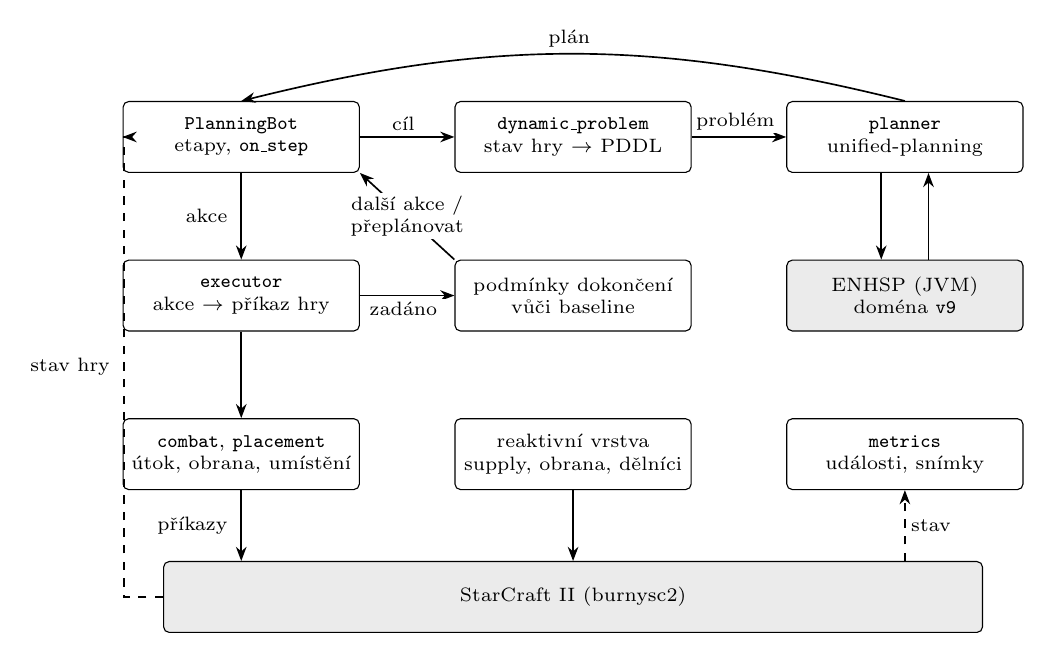
\begin{tikzpicture}[
		node distance=11mm and 12mm,
		box/.style={draw, rounded corners=2pt, align=center, font=\scriptsize,
			minimum width=30mm, minimum height=9mm, inner sep=2pt},
		ext/.style={box, fill=black!8},
		flow/.style={-{Stealth[length=1.8mm]}, semithick},
		obs/.style={flow, dashed},
		lbl/.style={font=\scriptsize, align=center, fill=white, inner sep=1pt},
	]

	% columns: planning | problem and verification | planner and reactive layer
	\node[box] (bot) {\texttt{PlanningBot}\\ etapy, \texttt{on\_step}};
	\node[box, right=of bot] (problem) {\texttt{dynamic\_problem}\\ stav hry $\to$ PDDL};
	\node[box, right=of problem] (planner) {\texttt{planner}\\ unified-planning};

	\node[box, below=of bot] (exec) {\texttt{executor}\\ akce $\to$ příkaz hry};
	\node[box, below=of problem] (gate) {podmínky dokončení\\ vůči baseline};
	\node[ext, below=of planner] (enhsp) {ENHSP (JVM)\\ doména \texttt{v9}};

	\node[box, below=of exec] (combat) {\texttt{combat}, \texttt{placement}\\ útok, obrana, umístění};
	\node[box, below=of gate] (reactive) {reaktivní vrstva\\ supply, obrana, dělníci};
	\node[box, below=of enhsp] (metrics) {\texttt{metrics}\\ události, snímky};

	\node[ext, below=9mm of reactive, minimum width=104mm] (sc2) {StarCraft~II (burnysc2)};

	% planning
	\draw[flow] (bot) -- node[lbl, above=1pt] {cíl} (problem);
	\draw[flow] (problem) -- node[lbl, above=1pt] {problém} (planner);
	\draw[flow] ([xshift=-3mm]planner.south) -- ([xshift=-3mm]enhsp.north);
	\draw[flow] ([xshift=3mm]enhsp.north) -- ([xshift=3mm]planner.south);
	\draw[flow] (planner.north) to[bend right=14] node[lbl, above=1pt] {plán} (bot.north);

	% execution
	\draw[flow] (bot) -- node[lbl, left=1pt] {akce} (exec);
	\draw[flow] (exec) -- node[lbl, below=1pt] {zadáno} (gate);
	\draw[flow] (gate.north west) -- node[lbl, pos=0.5] {další akce /\\ přeplánovat} (bot.south east);
	\draw[flow] (exec) -- (combat);
	\draw[flow] (combat) -- node[lbl, left=1pt] {příkazy} (combat |- sc2.north);
	\draw[flow] (reactive) -- (sc2.north -| reactive);

	% observation
	\draw[obs] (sc2.north -| metrics) -- node[lbl, right=1pt] {stav} (metrics);
	\draw[obs] (sc2.west) -- ++(-5mm,0) |- node[lbl, pos=0.25, left=1pt] {stav hry} (bot.west);
\end{tikzpicture}

	\caption[Architektura agenta.]{Architektura agenta. Plné šipky jsou tok řízení, čárkované tok pozorování. Šedé bloky jsou externí systémy.}
	\label{fig:architektura}
\end{figure}

Oproti~\cite{Orava2025} se architektura liší ve dvou bodech. Plánovač dostává úplný numerický stav (suroviny, toky, kapacity), ne jen fakta o~existenci budov, a~akce se neodškrtává zadáním příkazu, ale až potvrzeným účinkem. Druhý bod je nutný právě kvůli prvnímu: numerický plán obsahuje předpoklady o~tom, kolik surovin v~kterém okamžiku bude, a~ty musí vykonávání dodržet, jinak se plán a~hra rozejdou (sekce~\ref{sec:limity}).

\section{Numerická doména}
\label{sec:domena}

Doména \texttt{sc2-terran-macro} je zapsána v~PDDL~2.1 úrovně~2 a~deklaruje jen požadavky \texttt{:typing} a~\texttt{:numeric-fluents}. Nemá objekty ani predikáty: veškerý stav je ve 24~numerických fluentech (tabulka~\ref{tab:fluenty}) a~akce jsou bez parametrů. Volba počtů místo objektů je záměrná. Agent nepotřebuje rozlišovat jednotlivé budovy téhož typu, protože výběr konkrétní budovy, na kterou se příkaz zadá, je úlohou vykonávací vrstvy, a~akce bez parametrů nemusí plánovač instancovat přes všechny objekty, takže groundovaný problém zůstává malý bez ohledu na velikost armády.

\begin{table}[ht]
	\centering
	\caption{Fluenty domény \texttt{domain\_numeric\_v11.pddl}.}
	\label{tab:fluenty}
	\begin{tabularx}{\textwidth}{@{} l >{\raggedright\arraybackslash}X @{}}
		\toprule
		\textbf{Skupina} & \textbf{Fluenty} \\
		\midrule
		Suroviny a~toky & \texttt{minerals}, \texttt{vespene}, \texttt{mining-rate}, \texttt{gas-rate} \\
		Supply & \texttt{supply-used}, \texttt{supply-cap} \\
		Budovy & \texttt{depot-count}, \texttt{barracks-count}, \texttt{refinery-count}, \texttt{factory-count}, \texttt{engineeringbay-count}, \texttt{cc-count}, \texttt{techlab-barracks-count}, \texttt{techlab-factory-count} \\
		Armáda & \texttt{marine-count}, \texttt{marauder-count}, \texttt{tank-count} \\
		Technologie & \texttt{weapon-upgrades}, \texttt{armor-upgrades}, \texttt{stimpack} \\
		Výrobní kapacita & \texttt{rax-time}, \texttt{factory-time} \\
		Útok & \texttt{attacks-launched}, \texttt{attack-threshold} \\
		\bottomrule
	\end{tabularx}
\end{table}

Doména má 16~akcí (tabulka~\ref{tab:akce}). Ceny všech akcí odpovídají cenám, které hra skutečně účtuje; kontroluje to automatický test, který z~domény vyčte efekty \texttt{decrease} nad fluenty \texttt{minerals} a~\texttt{vespene} a~porovná je s~tabulkou cen hry (\texttt{tests/test\_domain\_costs.py}). Test vznikl poté, co se ukázalo, že všechny verze až po čtvrtou účtovaly stavbu Factory bez jejích 100~jednotek plynu (sekce~\ref{sec:vyvoj}).

\begin{table}[ht]
	\centering
	\caption[Akce domény \texttt{domain\_numeric\_v11.pddl}.]{Akce domény \texttt{domain\_numeric\_v11.pddl}. Cena je v~minerálech/plynu; všechny akce kromě akcí čekání navíc vyžadují \texttt{(< (attacks-launched) 1)}.}
	\label{tab:akce}
	\footnotesize
	\begin{tabularx}{\textwidth}{@{} l r >{\raggedright\arraybackslash}X >{\raggedright\arraybackslash}X @{}}
		\toprule
		\textbf{Akce} & \textbf{Cena} & \textbf{Další předpoklady} & \textbf{Efekty mimo cenu} \\
		\midrule
		\texttt{wait\_for\_minerals} & -- & -- & $+$\texttt{mining-rate} minerálů, $+$\texttt{gas-rate} plynu, $+5$\,s výroby na budovu \\
		\texttt{wait\_for\_vespene} & -- & Refinery & totéž \\
		\texttt{build\_supply\_depot} & 100/0 & cap $\le 192$, volné supply $< 16$ & cap $+8$ \\
		\texttt{build\_barracks} & 150/0 & depot, Barracks $< 4\cdot$CC & Barracks $+1$ \\
		\texttt{build\_refinery} & 75/0 & Refinery $< 2\cdot$CC & \texttt{gas-rate} $+25$ \\
		\texttt{expand} & 400/0 & CC $< 3$ & CC $+1$, \texttt{mining-rate} $+40$ \\
		\texttt{build\_factory} & 150/100 & Barracks, Factory $<$ CC & Factory $+1$ \\
		\texttt{build\_engineeringbay} & 125/0 & depot, žádná EBay & EBay $+1$ \\
		\texttt{build\_techlab\_barracks} & 50/25 & Barracks bez add-onu & Tech Lab $+1$ \\
		\texttt{build\_techlab\_factory} & 50/25 & Factory bez add-onu & Tech Lab $+1$ \\
		\texttt{train\_marine} & 50/0 & Barracks, \texttt{rax-time} $\ge 18$, 1~supply & Marine $+1$ \\
		\texttt{train\_marauder} & 100/25 & Tech Lab, \texttt{rax-time} $\ge 21$, 2~supply & Marauder $+1$ \\
		\texttt{train\_siegetank} & 150/125 & Tech Lab u~Factory, \texttt{factory-time} $\ge 32$, 3~supply & Tank $+1$ \\
		\texttt{research\_weapons} & 100/100 & EBay, úroveň $< 1$ & úroveň $+1$ \\
		\texttt{research\_stimpack} & 100/100 & Tech Lab u~Barracks & Stimpack \\
		\texttt{attack} & -- & hodnota armády $\ge$ \texttt{attack-threshold} & armáda $:= 0$, \texttt{attacks-launched} $+1$ \\
		\bottomrule
	\end{tabularx}
\end{table}

Model zjednodušuje hru v~několika ohledech, které je třeba znát při čtení výsledků. Doména neobsahuje dělníky jako akci; rychlost těžby se před každým plánováním odvozuje z~jejich skutečného počtu a~nová základna nebo Refinery ji zvýší pevným odhadem (\texttt{mining-rate} $+40$, \texttt{gas-rate} $+25$). Expanze je omezena na tři základny. Engineering Bay vyžaduje v~modelu Supply Depot, ač ve hře stačí Command Center. Fluent \texttt{armor-upgrades} je deklarován, ale žádná akce ho nemění, a~výzkum zbraní je jen jedné úrovně, protože Armory potřebná pro další úrovně v~modelu není. Limity výroby (nejvýše čtyři Barracks a~jedna Factory na základnu, jedna Engineering Bay, depoty jen do kapacity 192 a~jen při méně než 16~volných supply) nejsou pravidla hry, ale ořez stavového prostoru: bez nich plánovač stavěl budovy, které pak neměl čím zaplnit, a~s~příliš těsnými limity zase neměl za co utratit nastřádanou banku (sekce~\ref{sec:vyvoj}).

Akce \texttt{attack} (výpis~\ref{lst:attack}) vyžaduje, aby vážená hodnota armády, Marine~1, Marauder~2 a~Siege Tank~3, dosáhla prahu \texttt{attack-threshold}, a~armádu \enquote{spotřebuje}: vynuluje počty jednotek a~zvýší počet vyslaných útoků. Protože všechny ostatní akce kromě čekání vyžadují \texttt{(< (attacks-launched) 1)}, je útok v~každém plánu nejvýše jeden a~je jeho poslední akcí; vše, co plán postaví a~vytrénuje, se odehraje před ním.

\begin{lstlisting}[caption={Akce útoku v~doméně v11.},label=lst:attack,float,basicstyle=\ttfamily\small]
(:action attack
  :parameters ()
  :precondition (and (< (attacks-launched) 1)
    (>= (+ (marine-count) (+ (* 2 (marauder-count))
                             (* 3 (tank-count))))
        (attack-threshold)))
  :effect (and (assign (marine-count) 0)
               (assign (marauder-count) 0)
               (assign (tank-count) 0)
               (increase (attacks-launched) 1)))
\end{lstlisting}

\section{Modelace času}
\label{sec:cas}

Doména neobsahuje durativní akce; čas do ní vstupuje dvěma akcemi čekání (výpis~\ref{lst:wait}). Jedna akce čekání představuje pevný úsek $\Delta = 5$~herních sekund (\texttt{WAIT\_SECONDS}) a~přičte k~fluentům to, co se za tento úsek nastřádá: minerály podle \texttt{mining-rate}, plyn podle \texttt{gas-rate} a~výrobní sekundy podle počtu výrobních budov. Plán je díky tomu nejen pořadím akcí, ale i~hrubým rozvrhem: počet akcí čekání mezi dvěma akcemi říká, kolik herního času mezi nimi uplyne, než si je agent může dovolit.

\begin{lstlisting}[caption={Akce čekání (\enquote{hodiny}) v~doméně v11.},label=lst:wait,float,basicstyle=\ttfamily\footnotesize]
(:action wait_for_minerals
  :parameters () :precondition ()
  :effect (and (increase (minerals) (mining-rate))
               (increase (vespene) (gas-rate))
               (increase (rax-time) (* 5 (barracks-count)))
               (increase (factory-time) (* 5 (factory-count)))))
\end{lstlisting}

\paragraph{Rychlost těžby.} Hodnoty \texttt{mining-rate} a~\texttt{gas-rate} jsou množství suroviny, které hra skutečně vytěží za $\Delta$, a~počítají se z~dělníků právě přiřazených k~těžbě:
\[
	\texttt{mining-rate} = \left\lfloor \Delta \cdot r_m \cdot \sum_{b} \min(h_b, 16) \right\rfloor,
	\qquad
	\texttt{gas-rate} = \left\lfloor \Delta \cdot r_g \cdot \sum_{r} h_r \right\rfloor,
\]
kde $h_b$ je počet dělníků na minerálech u~základny~$b$, $h_r$ počet dělníků u~Refinery~$r$ a~$r_m = 0{,}93$ a~$r_g = 0{,}84$ jsou rychlosti těžby jednoho dělníka za sekundu. Hodnota~$r_g$ byla kalibrována podle her sérií T8.1 a~T8.2 a~platí od verze~7 domény (\serie{T8.2_v7_medium}). Při dvanácti dělnících na začátku hry vychází 55~minerálů na jedno čekání. Obě hodnoty jsou nejméně~1, protože akce s~nulovým přírůstkem nic nemění a~plánovač by problém, ve kterém je potřeba čekat, prohlásil za neřešitelný. Stejnou funkci používá i~vykonávací vrstva, když rozhoduje, zda čekání skončilo, takže to, co předpokládá doména, a~to, co se ve hře testuje, se nemůže rozejít.

\paragraph{Výrobní kapacita.} Od verze~6 nese doména dva fluenty výrobního času, \texttt{rax-time} a~\texttt{factory-time}: kolik sekund výroby mají Barracks, resp. Factory k~dispozici. Každé čekání přidá 5~s za každou výrobní budovu a~trénink jednotky spotřebuje její dobu výroby (Marine~18~s, Marauder~21~s, Siege Tank~32~s). Na začátku plánu se fluenty nastaví podle budov, které jsou právě volné. Plán, který chce utratit velkou banku rychle, tak musí postavit víc výrobních budov; jinak by mohl naplánovat dvacet tanků z~jedné Factory, které by se ve hře vyráběly déle než deset minut. Model je přitom hrubý: výrobní čas \texttt{rax-time} roste o~5~s za \emph{každé} Barracks, i~když Marauder potřebuje Barracks s~Tech Labem. Plánovač proto může počítat s~Maraudery ze všech Barracks, zatímco hra je vyrábí jen u~jednoho; v~hlavní sérii proti VeryEasy to ve dvou hrách vedlo k~plánům s~25 a~28~Maraudery, které držely armádu doma přes deset minut (sekce~\ref{sec:vs-ai}).
% TODO (T4.9): doménu v12 s výrobním časem Tech Labů doplnit, až bude změřena.

\paragraph{Jedny hodiny.} Ve verzi~6 přičítala akce \texttt{wait\_for\_vespene} jen plyn a~výrobní čas, nikoli minerály vytěžené za stejnou dobu, a~plánovač ji používal jako levný zdroj výrobního času. Od verze~7 přičítají obě akce čekání všechny tři veličiny současně; liší se jen tím, že \texttt{wait\_for\_vespene} vyžaduje Refinery. Model má tedy jedny hodiny a~každé čekání je pět sekund pro celou ekonomiku.

\paragraph{Proč ne durativní akce.} Spojitý model těžby, buď durativní akcí se spojitým efektem \texttt{(increase (minerals) (* \#t (mining-rate)))}, nebo procesem PDDL+~\cite{FoxLong2006}, by byl věrnější: plán by byl rozvrhem s~makespanem a~čekání by nebylo třeba plánovat. Diskrétní hodiny byly zvoleny ze tří důvodů. Plán zůstává posloupností okamžitých akcí, takže vykonávání i~podmínky dokončení jsou jednoduché a~každou akci čekání lze ve hře přímo ověřit. Na doménu stačí plánovač úrovně~2, kterých je víc a~jsou rychlejší než plánovače se spojitým časem. A~rozlišení pěti sekund je vůči době výroby jednotek (18 až 32~s) a~staveb (desítky sekund) dostatečně jemné. Cenou je délka plánů: akce čekání tvoří velkou část každého plánu (na pevných problémech etap 0 až 2 jde o~18 z~28, 14 z~26 a~18 z~36 akcí, \serie{T5.4_planners_offline}) a~vyhovující plánovač bez metriky někdy čeká víc, než je nutné. Akce čekání přitom nelze z~domény odstranit: bez nich by čísla v~doméně jen omezovala pořadí akcí a~numerický model by se zredukoval na klasický.

Spojitou variantu práce ověřila mimo hru. Doména \texttt{domain\_temporal.pddl} je doména v11 zapsaná v~PDDL+: akce čekání nahrazuje proces, který po celou dobu spojitě zvyšuje suroviny a~výrobní čas, a~ENHSP ji plánuje s~rozhodovacím krokem 1~s. Na pevných problémech etap 0 až 2 našel plány za přibližně 0,6~s s~délkou rozvrhu (\emph{makespan}) 76, 73 a~122~herních sekund, zatímco diskrétní plány téhož plánovače odpovídají 90, 70 a~90~sekundám (\serie{T5.4_planners_offline}). Spojitý model je tedy řešitelný stejně rychle; v~etapě~0 dává kratší plán, v~etapě~2 delší, protože obě varianty hledají vyhovující, nikoli nejkratší plán. Ve hře se spojitá varianta nepoužívá: plán s~časovými značkami by vyžadoval jiný druh vykonávání, který akce nespouští po jedné, ale podle času, a~ten práce neimplementuje. Ani jedna z~variant zatím nemodeluje dobu staveb a~výzkumů; ve hře se to projevuje například tím, že depot přidá supply v~modelu okamžitě, ve hře až po 21~s stavby (\serie{T4.8_supply_wait_veryeasy}). Spojitý čas by takové trvání vyjádřit uměl, což je přirozené pokračování práce.

\section{Etapové cíle a~generování problému}
\label{sec:etapy}

Hra je rozdělena do čtyř etap s~cíli v~tabulce~\ref{tab:etapy}. Etapy 0 až 2 budují technologii a~armádu po krocích, které odpovídají technologickému stromu; etapa~3 je poslední a~opakuje se. Její cíl \texttt{(>= (attacks-launched) 1)} je splněn akcí \texttt{attack} a~generátor problému nastavuje \texttt{attacks-launched} vždy na~0, takže cíl znamená \enquote{vyšli ještě jednu vlnu}. Aby plánovač mohl zaútočit, musí nejprve postavit armádu s~hodnotou alespoň \texttt{attack-threshold}; po vyčerpání plánu se etapa~3 naplánuje znovu. Pozdní hra je tak cyklem shromáždění, útoku a~nového shromáždění, o~jehož načasování i~složení rozhoduje plánovač.

\begin{table}[ht]
	\centering
	\caption{Etapové cíle (\texttt{STAGE\_GOALS}).}
	\label{tab:etapy}
	\begin{tabularx}{\textwidth}{@{} c >{\raggedright\arraybackslash}X @{}}
		\toprule
		\textbf{Etapa} & \textbf{Cíl} \\
		\midrule
		0 & $\ge 1$ Barracks, $\ge 6$ Marine \\
		1 & $\ge 1$ Refinery, $\ge 1$ Tech Lab u~Barracks, $\ge 4$ Marauder, $\ge 8$ Marine \\
		2 & $\ge 1$ Factory, $\ge 1$ Tech Lab u~Factory, $\ge 2$ Siege Tank, zbraně úrovně~1, Stimpack, $\ge 14$ Marine \\
		3 (opakuje se) & $\ge 1$ vyslaný útok \\
		\bottomrule
	\end{tabularx}
\end{table}

\paragraph{Strop banky.} Samotné cíle etap neříkají nic o~surovinách, které agent nastřádal navíc. Kdyby plánovač jen splnil cíl, banka by rostla, což je stagnace popsaná v~\cite{Orava2025}. Každý cíl je proto rozšířen o~podmínku na zůstatek minerálů na konci plánu:
\[
	\textit{cíl etapy} \wedge \big(\texttt{supply-used} \ge 190 \vee \texttt{minerals} \le c\big).
\]
Agent nejprve plánuje s~přísným stropem $c = 400$, takže plán musí utratit celou banku nad tento zůstatek a~rozhodnout, za co. Když pro přísný cíl plán nenajde, zkusí slabší strop $c = \max(400,\; m_0 - 1\,500)$, kde $m_0$ je stav banky při plánování, tedy utratit nejvýše 1\,500~minerálů. Do verze kódu, na které běžely série T8, platil jen slabší strop; část příjmu jednoho plánovacího cyklu pak v~bance zůstávala (\serie{T4.8_spend_bank_veryeasy}). Podmínka odpadá, když už se do supply nevejdou další jednotky. Na plyn strop není: s~několika Refinery přinese každé čekání zhruba tolik plynu, kolik jednotka stojí, takže plynový strop byl nedosažitelný a~prodlužoval plány na stovky akcí (\serie{T8.3_v8_medium}).

\paragraph{Práh útoku.} Útok vyžaduje armádu s~hodnotou 30. Jednotky vyslané do útoku ale dál drží supply, a~když armáda v~poli zabírá většinu kapacity, doma se armáda s~hodnotou 30 postavit nedá a~plánovač by marně hledal plán, dokud nevyprší limit. Generátor problému proto nastavuje
\[
	\texttt{attack-threshold} = \max\big(0, \min(30,\; v_{\mathrm{doma}} + c_{\mathrm{dosažitelná}} - \texttt{supply-used})\big),
\]
kde $v_{\mathrm{doma}}$ je hodnota armády u~základen a~$c_{\mathrm{dosažitelná}}$ kapacita supply, kterou lze ještě postavit depoty (193 až 200 podle aktuální kapacity). Když je práh nulový, nevejde se doma nic a~cílem etapy~3 je jen jedno čekání.

Problém PDDL vzniká přímo z~pozorování: každý fluent je funkcí stavu hry (počty budov a~jednotek, banka, rychlosti těžby, volné výrobní budovy). Armáda se počítá jen z~jednotek, které jsou u~základen a~nebyly vyslány do probíhajícího útoku; ty už plánovač nevidí (sekce~\ref{sec:vykonavani}). Generátor zapisuje jen fluenty, které daná doména deklaruje, takže agent může hrát s~libovolnou starší verzí domény, což je podmínkou reprodukovatelnosti historických sérií.

\section{Vykonávací vrstva}
\label{sec:vykonavani}

Vykonávací vrstva odděluje dvě otázky: zda lze akci \emph{zadat} a~zda se akce \emph{dokončila}. Na první odpovídá \texttt{executor}: vrátí, zda příkaz zadal, a~pokud ne, uvede důvod (například \enquote{cannot afford}, \enquote{no free geyser}). Důvod začínající slovem \texttt{waiting} znamená, že akce jen čeká na dokončení rozestavěné budovy nebo na uvolnění fronty, což je postup, nikoli selhání.

Na druhou otázku odpovídá \emph{podmínka dokončení} (tabulka~\ref{tab:podminky}). Podmínky se vyhodnocují proti \emph{baseline}, stavu zachycenému těsně před zadáním akce. Díky tomu plán se čtyřmi akcemi \texttt{build\_supply\_depot} postaví čtyři depoty, a~ne jeden, který by splnil podmínku \enquote{nějaký depot existuje}, a~čekání skončí, až banka vzroste o~\texttt{mining-rate} proti stavu při zadání. Vykonávací vrstva tedy nikdy nepostoupí na základě předpokladu, že akce vyšla; vždy čeká, až to potvrdí hra.

\begin{table}[ht]
	\centering
	\caption{Podmínky dokončení akcí vůči baseline zachycené při zadání.}
	\label{tab:podminky}
	\begin{tabularx}{\textwidth}{@{} l >{\raggedright\arraybackslash}X @{}}
		\toprule
		\textbf{Akce} & \textbf{Akce je hotová, když} \\
		\midrule
		stavba, expanze, add-on & počet budov daného typu (hotových i~rozestavěných) přesáhl baseline \\
		trénink & počet jednotek daného typu (živých i~ve frontě) přesáhl baseline \\
		výzkum & vylepšení je dokončené nebo prokazatelně probíhá \\
		čekání & banka dosáhla stavu při zadání $+$ \texttt{mining-rate} (resp.\ \texttt{gas-rate}) \\
		útok & žádná z~vyslaných jednotek nestojí nečinně u~základen \\
		\bottomrule
	\end{tabularx}
\end{table}

\paragraph{Časové limity a~eskalace.} Zadaná akce, která se do 30~s nedokončí (například dělník zahynul cestou na staveniště), se uvolní a~zaznamená jako \texttt{action\_timeout}. Akci, kterou nelze zadat 30~s, řeší agent eskalací ve třech krocích: nejprve etapu přeplánuje z~aktuálního stavu, takže plánovač sám uvidí, co chybí, a~buď to postaví, nebo cíl obejde. Po třech takových přeplánováních bez mezilehlého postupu se další nevykonatelné akce vynechávají a~po dalších třech agent opustí celou etapu. Akce, která čeká jen na dokončení stavby, smí čekat až 120~s. Počítadlo pokusů se nuluje jen skutečným postupem, tedy zadáním nebo dokončením akce; nulování při vynechání dovolilo agentovi v~jedné z~dřívějších verzí donekonečna cyklit mezi dvěma nevykonatelnými akcemi.

\paragraph{Přeuspořádání plánu.} Plán se vykonává po jedné akci, ale hra některou akci často zadrží: Barracks pro Tech Lab se ještě staví, všechny výrobní fronty jsou plné, jednotka čeká na rozestavěný depot. Dokud se taková akce nedala zadat, stál celý plán; v~sérii proti VeryEasy na doméně v9 to bylo přibližně 290~s z~přibližně 810~s hry a~příjem těchto sekund model neviděl (\serie{T5.2_VeryEasy}). Když vykonávací vrstva hlásí, že akce jen čeká, posune agent před ni první pozdější akci téhož plánu, ale jen tehdy, když přeuspořádaný plán z~počátečního stavu problému podle simulátoru knihovny unified-planning stále projde všemi předpoklady a~skončí v~cíli (modul \texttt{plan\_order}). Akce čekání se nepřesouvají. Agent tak nerozhoduje o~ničem novém: mění se jen pořadí akcí, které vybral plánovač, a~jen tam, kde to dovoluje jeho vlastní model. Každý posun se zaznamená jako \texttt{plan\_reordered}.

\paragraph{Selhání plánovače.} Agent zkouší cíle od nejsilnějšího: nejprve cíl s~přísným stropem banky, potom se slabším (sekce~\ref{sec:etapy}). Pro každý cíl spustí ENHSP ve výchozí konfiguraci ($h_{\mathrm{add}}$, GBFS) a~při vypršení časového limitu ještě jednou s~konfigurací $h_{\mathrm{mrp}}$ a~GBFS; během vývoje se ukázalo, že obě konfigurace selhávají na různých stavech. Teprve když plán nenajde žádná kombinace, přejde agent do nouzového režimu: trénuje Marine a~při šesti Marinech zaútočí. Nouzový režim je jediným místem, kde o~útoku nerozhoduje plánovač, a~každý neúspěšný pokus se zaznamená jako \texttt{planner\_error}.

\paragraph{Útok mimo plán.} Akce \texttt{attack} v~doméně armádu spotřebuje a~vykonávání to dodržuje doslova. Vykonávací vrstva útok zadá, až když ve hře platí jeho předpoklad z~modelu: hodnota armády u~základen dosáhla prahu, se kterým plán počítal. Trénink se totiž považuje za hotový už zařazením do fronty, takže část jednotek, se kterými plán počítal, ještě nemusí existovat; jednotky, které jsou při útoku stále ve výrobě, zůstanou doma pro další vlnu. Útok je hotový, jakmile všechny vyslané jednotky opustily základny; jejich identifikátory se uloží jako \emph{nasazené} a~plánovač je v~dalších problémech nevidí. Agent tak hned začne shromažďovat další vlnu, zatímco nasazené jednotky bojují mimo plán: postupují k~nejbližší známé budově soupeře, a~když žádnou neznají, prohledávají místa možných expanzí. Jakmile nasazené jednotky ztratí polovinu vyslané hodnoty, přeživší se vrátí domů a~připojí se k~další vlně. Rozhodnutí \emph{kdy} a~\emph{s~čím} zaútočit tedy patří plánovači; průběh boje je provedením tohoto rozhodnutí.

\section{Reaktivní vrstva}
\label{sec:reaktivni}

V~každém kroku hry před plánovací vrstvou běží čtyři reaktivní rutiny:
\begin{itemize}
	\item \textbf{rozdělování dělníků} na minerály a~plyn vestavěnou funkcí knihovny,
	\item \textbf{trénink dělníků} do saturace: 16 na Command Center a~3 na Refinery, nejvýše 66,
	\item \textbf{nouzový Supply Depot}, když zbývá méně než 2~volné supply a~žádný depot se nestaví,
	\item \textbf{obrana základny}: nepřátelské jednotky v~okruhu 35 od kterékoli vlastní základny napadne celá armáda, která je v~tom okruhu (jednotky útočící jinde se nevolají zpět); Siege Tanky se v~dosahu nepřítele rozloží.
\end{itemize}

Každá z~rutin řeší situaci, na kterou nelze čekat do dalšího plánu (sekce~\ref{sec:pozadavky}). Nouzový depot a~obrana se zaznamenávají jako \texttt{reactive\_override}, obrana jednou za střet, ne za každý krok hry, takže jejich rozsah je měřitelný: v~hlavní sérii proti obtížnosti Medium připadalo na hru v~průměru 219,8~zadaných akcí plánu a~24,1 takových zásahů (\serie{E5_numeric_Medium}). Rozdělování a~trénink dělníků se nezaznamenávají a~v~tomto poměru nejsou. Trénink dělníků je ze čtyř rutin nejméně obhajitelný, protože jde o~ekonomické rozhodnutí; jeho přesun do domény je otevřeným bodem (kapitola~\ref{chap:experimenty}).

\section{Vývoj domény v1--v11}
\label{sec:vyvoj}

Doména vznikala iterativně. Každá verze je samostatný soubor v~adresáři \texttt{planning/} (od \texttt{domain\_numeric.pddl} po \texttt{domain\_numeric\_v11.pddl}), vznikla jako odpověď na konkrétní pozorování z~her a~byla ověřena další sérií her. Tabulka~\ref{tab:vyvoj} shrnuje změny domény; změny vykonávací vrstvy v~rámci téže verze a~podrobný rozbor sérií proti obtížnosti Medium jsou v~kapitole~\ref{chap:experimenty}. Všechna čísla pocházejí z~uvedených sérií a~z~deníku experimentů \texttt{experiments/LOG.md}.

\begin{table}[p]
	\centering
	\caption[Vývoj numerické domény.]{Vývoj numerické domény. V~=~výhra, P~=~prohra, R~=~remíza (limit 1\,800 herních sekund); CI je 95\% Wilsonův interval.}
	\label{tab:vyvoj}
	\footnotesize
	\begin{tabularx}{\textwidth}{@{} c >{\raggedright\arraybackslash}X >{\raggedright\arraybackslash}X >{\raggedright\arraybackslash}p{3.6cm} @{}}
		\toprule
		\textbf{Verze} & \textbf{Změna} & \textbf{Výsledek} & \textbf{Série} \\
		\midrule
		v1 & 21 fluentů, 16 akcí; suroviny, supply, rychlosti těžby, počty budov a~jednotek & po opravách vykonávání výhry proti VeryEasy, v~etapě~3 se ale hromadí banka (4\,625 minerálů, 1\,344 plynu na konci hry) & \serie{2026-10-25_8d754f4}, \serie{2026-10-25_d8a042d} \\
		v2 & limity výroby, strop banky & etapa~3 vyrábí (Siege Tanky 0 $\to$ 12), banka ale roste dál (3\,975 $\to$ 5\,005 minerálů): jedna Factory nestačí, model nemá výrobní kapacitu & \serie{2026-10-25_e002cbb} \\
		v3 & zbraně jen 1.~úroveň, depot jen při $< 16$ volných supply; útok uvolňuje supply armády & hypotéza vyvrácena: model uvolnil supply, které přeživší armáda dál drží, a~jednotky byly odmítnuty při 77/79 supply & \serie{2026-10-26_8f239e5} \\
		v4 & útok supply neuvolňuje & výhry proti VeryEasy; porážka, když \texttt{build\_factory} odmítnuto při 3\,000 minerálech: doména neúčtovala plyn Factory & \serie{2026-10-26_bbf1fa4}, \serie{2026-10-26_06116be} \\
		v5 & Factory stojí 100 plynu; test všech cen & VeryEasy a~Easy 6/6~V; Medium 3~V / 6~P / 1~R, 30~\% (CI 11--60~\%); banka nad 500 minerály 87--95~\% hry & \serie{2026-10-30_T1.6_85bd1dc}, \serie{T8.1_medium} \\
		v6 & výrobní kapacita (\texttt{rax-time}, \texttt{factory-time}) & VeryEasy 3/3~V; recenze odhalila plynové čekání jako volný výrobní čas & \serie{T8.2_veryeasy}, \serie{T8.2_medium} \\
		v7 & jedny hodiny pro obě čekání, $r_g = 0{,}84$ & Medium 8~V / 2~P, 80~\% (CI 49--94~\%); medián délky hry 690~s (v5: 1\,063~s) & \serie{T8.2_v7_veryeasy}, \serie{T8.2_v7_medium} \\
		v8 & práh útoku 30 (dříve 20), útok končí plán & Medium 8~V / 0~P / 2~R, 80~\% (CI 49--94~\%), bez porážek & \serie{T8.3_v8_medium} \\
		v9 & práh útoku jako fluent omezený dosažitelným supply & Medium 4~V / 1~P, 80~\% (CI 38--96~\%) & \serie{T8.3_v9_medium}, \serie{T8.3_reachable_cap_medium} \\
		v10 & v9 $+$ \texttt{total-cost} pro pokusy s~metrikou plánu & metrika nezlepšila žádný plán; jen pro experimenty mimo hru & \serie{T4.2_planner_configs} \\
		v11 & Barracks $\le 4\cdot$CC, až 3~CC; plány utrácejí banku do 400 & VeryEasy 20/20~V; Medium 20/20 dokončených her~V, 3~starty zastaveny (sekce~\ref{sec:vs-ai}) & \serie{T4.8_spend_bank_veryeasy}, \serie{E5_numeric_VeryEasy}, \serie{E5_numeric_Medium} \\
		\bottomrule
	\end{tabularx}
\end{table}

Z~vývoje plynou dvě obecnější zjištění. Za prvé, většina verzí neopravovala plánovač, ale \emph{model}: chybějící cenu (v4 $\to$ v5), chybějící výrobní kapacitu (v5 $\to$ v6), nekonzistentní hodiny (v6 $\to$ v7). Teprve s~realistickým modelem kapacity a~času začal agent proti Medium vyhrávat většinu her. Za druhé, chyby modelu se projevovaly jako ekonomické symptomy, nejčastěji jako rostoucí banka, a~ty šly odhalit jen proto, že se ekonomika měřila (podíl hry s~bankou nad 500~minerály, hodnota armády v~čase). Stejný symptom, který~\cite{Orava2025} pozoruje jako stagnaci, je v~numerickém modelu diagnostickým signálem, který ukazuje na konkrétní chybějící část domény.

\section{Klasická doména pro ablaci}
\label{sec:klasicka}

Klasická doména \texttt{domain\_classical.pddl} slouží k~odpovědi na otázku, co přinášejí samotná čísla. Obsahuje stejné makroakce jako numerická doména kromě akcí čekání a~je zapsána v~propozičním stylu Oravovy domény~\cite{Orava2025}: každá budova a~jednotka je objekt, technologické předpoklady jsou existenční kvantifikátory a~stav jsou predikáty (\texttt{built}, \texttt{has-techlab}, \texttt{trained}, \texttt{weapons-researched}, \texttt{stim-researched}, \texttt{attacked}). Supply je zásobník slotů po dvou supply: každý depot \enquote{odemkne} čtyři sloty a~jednotka obsadí jeden slot bez ohledu na velikost. Suroviny, rychlosti těžby a~výrobní kapacita v~doméně nejsou a~cenu akcí hlídá až vykonávací vrstva, která příkaz odmítne, dokud na něj banka nestačí.

Generátor problému \texttt{classical\_problem.py} převádí stav hry na objekty a~fakta a~numerické etapové cíle na objekty, které je třeba postavit nebo vytrénovat; limity výroby verze~2 jsou vyjádřeny počtem deklarovaných objektů budov. Útočná vlna etapy~3 má pevné složení s~hodnotou 30 (12~Marine, 6~Marauder, 2~Siege Tanky), zmenšené stejně jako práh numerické domény, když se doma nevejde; vykonávací vrstva pak útok zadá při hodnotě této vlny. Plánovačem je Fast Downward v~konfiguraci LAMA-first, stejně jako v~\cite{Orava2025}. Vykonávací vrstva, podmínky dokončení, reaktivní vrstva i~metriky jsou sdílené, takže srovnání numerického a~klasického agenta se liší jen modelem a~plánovačem. Klasický agent je funkční: proti úrovni VeryEasy vyhrál kontrolní hru v~čase 744~s s~mediánem 13~akcí na plán (\serie{T4.1_classical_check}); systematické srovnání je v~kapitole~\ref{chap:experimenty}.

\chapter{Implementace}
\label{chap:implementace}

Tato kapitola popisuje implementaci agenta a~experimentální infrastruktury: použité technologie, strukturu kódu a~řídicí smyčku, převod akcí na příkazy hry, měření a~dávkové spouštění her, problémy prostředí, které bylo třeba vyřešit, a~testování bez spuštěné hry. Zdrojový kód je na přiloženém médiu, jehož obsah je uveden na konci práce; popis odpovídá verzi \texttt{a3cb452}, na které běží hlavní série experimentů.

\section{Technologie}
\label{sec:technologie}

Agent je napsán v~Pythonu~3.14. Rozhraní hry zprostředkovává knihovna burnysc2~7.2.1~\cite{BurnySc2}, plánovač se volá přes unified-planning~1.3.0~\cite{Micheli2025} s~balíčky \texttt{up-enhsp}~0.1.1 (ENHSP) a~\texttt{up-fast-downward}~0.5.2 (klasická varianta). ENHSP běží v~JVM a~vyžaduje Javu ve verzi alespoň~17; vývoj probíhal s~OpenJDK~25. Pro sledování hry v~průběhu slouží jednoduchý webový panel ve frameworku Flask, testy používají pytest a~běží při každém nahrání změn v~GitHub Actions. Závislosti nutné pro běh agenta jsou s~přesnými verzemi v~\texttt{requirements.txt}, vývojové (Fast Downward, pytest) v~\texttt{requirements-dev.txt}. Vývojové série se hrály na mapě AcropolisLE z~oficiálního balíčku map, hlavní série na mapě Abyssal Reef LE, kterou používá i~\cite{Orava2025} a~která je převzata z~přílohy jeho práce (adresář \texttt{maps/}).

\section{Struktura kódu a~tok řízení}
\label{sec:struktura}

Tabulka~\ref{tab:moduly} shrnuje moduly. Všechny cesty k~souborům jsou odvozeny od umístění zdrojového souboru, takže agenta lze spustit z~libovolného adresáře, což využívá dávkové spouštění her.

\begin{table}[ht]
	\centering
	\caption{Moduly agenta a~experimentální infrastruktury.}
	\label{tab:moduly}
	\footnotesize
	\begin{tabularx}{\textwidth}{@{} l >{\raggedright\arraybackslash}X @{}}
		\toprule
		\textbf{Modul} & \textbf{Odpovědnost} \\
		\midrule
		\texttt{run.py} & vstupní bod: konfigurace hry z~příkazové řádky, spuštění hry, uložení výsledku \\
		\texttt{bot/planning\_bot.py} & třída \texttt{PlanningBot}: etapy, cíle, plánování, vykonávání a~podmínky dokončení, reaktivní vrstva \\
		\texttt{bot/executor.py} & převod akce PDDL na příkaz rozhraní hry, důvod odmítnutí \\
		\texttt{bot/placement.py} & umístění budov u~hlavní základny \\
		\texttt{bot/combat.py} & provedení útoku a~obrany \\
		\texttt{planning/dynamic\_problem.py} & stav hry $\to$ problém PDDL, rychlosti těžby, hodnota armády, práh útoku \\
		\texttt{planning/classical\_problem.py} & stav hry $\to$ problém klasické domény \\
		\texttt{planning/planner.py} & spuštění ENHSP, resp.\ Fast Downward přes unified-planning, časový limit, konfigurace ENHSP \\
		\texttt{planning/plan\_order.py} & přeuspořádání zbytku plánu, pokud je podle simulátoru stále platný \\
		\texttt{planning/*.pddl} & všechny verze numerické domény, klasická doména a~varianta v~PDDL+ \\
		\texttt{utils/metrics.py} & záznam událostí a~snímků hry \\
		\texttt{experiments/} & dávkové spouštění a~noční fronta sérií, agregace, grafy, srovnání plánovačů mimo hru, Oravův agent v~téže infrastruktuře \\
		\texttt{tests/} & testy bez hry, simulovaný stav hry, pevné problémy \\
		\bottomrule
	\end{tabularx}
\end{table}

Knihovna burnysc2 volá v~každém kroku hry asynchronní metodu \texttt{on\_step}. Její průběh ukazuje výpis~\ref{lst:onstep}: nejprve reaktivní vrstva a~sledování nasazených jednotek, potom měření a~nakonec nejvýše jeden krok plánu. Plánování probíhá synchronně uvnitř kroku; v~krokovém režimu (\texttt{realtime=False}) na něj hra čeká, takže doba výpočtu plánu se měří, ale herní čas nespotřebovává (sekce~\ref{sec:sc2}).

\begin{lstlisting}[caption={Řídicí smyčka agenta (zjednodušeno).},label=lst:onstep,float,basicstyle=\ttfamily\small,mathescape=true]
on_step():
    distribute_workers(); train_scvs()          # reaktivni vrstva
    manage_supply(); defend_base()
    follow_attack()                             # nasazene jednotky
    metrics.snapshot_if_due()                   # kazdych 10 hernich s
    if plan vycerpan:
        stage $\leftarrow$ min(stage + 1, 3); advance_plan(); return
    a $\leftarrow$ plan[index]
    if not issued:
        baseline $\leftarrow$ snapshot_baseline(a)    # pred zadanim
        if execute_action(a): issued $\leftarrow$ True
        elif akce jen ceka: pull_forward(a)        # preusporadani
        elif vyprsel limit pro zadani: handle_unissuable(a)
    elif COMPLETION_CONDITIONS[a](baseline):
        index $\leftarrow$ index + 1; issued $\leftarrow$ False
\end{lstlisting}

Metoda \texttt{advance\_plan} sestaví cíl etapy, zapíše problém a~zavolá plánovač. Plán spolu s~načteným problémem uloží do objektu \texttt{PlanOrder}, který umí ověřit přeuspořádání (sekce~\ref{sec:vykonavani}), a~akce převede na jejich jména (\texttt{build\_barracks}), podle kterých se hledá větev vykonávací vrstvy i~podmínka dokončení. Každé naplánování se zaznamená jako událost \texttt{plan\_generated} s~etapou, pořadím pokusu, dobou výpočtu, stavem plánovače, délkou plánu a~počtem akcí čekání. Baseline se zachycuje \emph{před} zadáním akce, protože zadaná stavba se ve hře okamžitě objeví jako rozestavěná a~baseline zachycená po zadání by ji už obsahovala a~nikdy by nebyla překročena.

\section{Překlad akcí na příkazy hry}
\label{sec:preklad}

Funkce \texttt{execute\_action} rozpozná akci podle jména a~zadá odpovídající příkaz. Pro každou akci řeší, \emph{kde} a~\emph{čím} ji provést, což doména záměrně nemodeluje:
\begin{itemize}
	\item \textbf{Trénink} se zadá u~výrobní budovy s~nejvolnější frontou; Marine přednostně u~Barracks bez add-onu, Marauder a~Siege Tank jen u~budovy s~Tech Labem, protože budova bez něj příkaz tiše zahodí. Fronta pojme nejvýše dvě jednotky: zařazením se jednotka zaplatí, takže banka sleduje plán a~nečeká na uvolnění budovy. Plná fronta je důvodem typu \texttt{waiting}, ne selháním, a~stejně tak chybějící supply, když se právě staví depot: knihovna burnysc2 počítá supply jako součást ceny, takže by jinak jednotku odmítla jako nezaplatitelnou.
	\item \textbf{Add-on} se staví jen u~hotové, nečinné výrobní budovy, a~to až po ověření, že je vedle ní místo; hra příkaz bez místa také tiše zahodí. Rozestavěná budova znamená čekání, nikoli selhání.
	\item \textbf{Refinery} se staví na nejbližším volném gejzíru u~hotové základny, \textbf{expanze} na nejbližším volném místě pro základnu.
	\item \textbf{Útok} se zadá, až když hodnota armády u~základen dosáhla prahu, se kterým plán počítal (sekce~\ref{sec:vykonavani}); vyšle všechny jednotky u~základen, které ještě nebyly nasazeny.
	\item \textbf{Čekání} nevyžaduje žádný příkaz, hra těží sama; zadání vždy uspěje a~celou práci dělá podmínka dokončení.
\end{itemize}

\paragraph{Umístění budov.} Ostatní budovy (Supply Depot, Barracks, Factory, Engineering Bay i~nouzový depot reaktivní vrstvy) umísťuje modul \texttt{placement}. Hledá místo v~okruhu 14~polí od hlavní základny a~dodržuje čtyři pravidla: budova stojí celá mimo stranu základny s~minerály a~plynem (dokud zbývá jiné místo), kolem každé budovy i~add-onu zůstává průchod šířky jednoho pole, místo pro add-on vedle Barracks a~Factory se nezastavuje a~nezastavuje se ani plocha přislíbená budově, ke které dělník teprve jde (rezervace platí 20~s, protože hra objednanou budovu do příchodu dělníka nevidí). Pravidla vznikla po hře, ve které depoty zastavily místo pro Tech Lab (sekce~\ref{sec:limity}). Test \texttt{test\_base\_layout.py} postaví na modelu mapy celé stavební pořadí a~prohledáváním do šířky ověří, že žádná budova není obestavěna a~že cesty dělníků ke gejzírům se nezměnily.

\section{Měření a~experimentální infrastruktura}
\label{sec:harness}

\paragraph{Konfigurace a~výsledek hry.} Skript \texttt{run.py} sestaví z~příkazové řádky konfiguraci hry: obtížnost a~rasu soupeře, mapu, doménu, plánovač a~jeho nastavení, časový limit a~semínko náhodného generátoru (náhodné, není-li zadáno, ale vždy zaznamenané). Spolu s~ní uloží i~verzi kódu, tj.~zkrácený hash commitu s~příznakem \texttt{-dirty}, pokud se sledované soubory liší od commitu. Výsledkem hry je soubor JSON, který obsahuje konfiguraci, časovou řadu událostí a~snímky stavu; vedle něj se ukládá záznam hry (\emph{replay}), který lze ve hře přehrát.

\paragraph{Události a~snímky.} Události zaznamenávají život plánu (\nolinkurl{plan_generated}, \nolinkurl{plan_issued}, \nolinkurl{plan_completed}), potíže (\nolinkurl{action_unissuable}, \nolinkurl{action_skipped}, \nolinkurl{action_timeout}, \nolinkurl{planner_error}), přeuspořádání (\nolinkurl{plan_reordered}), útoky (\nolinkurl{attack_retarget}, \nolinkurl{attack_resolved}), zásahy reaktivní vrstvy (\nolinkurl{reactive_override}) a~konec hry. Snímek se pořizuje každých 10~herních sekund a~obsahuje suroviny, supply, počty dělníků a~bojových jednotek, hodnotu armády, hotové budovy podle typu a~podíl dosavadní hry, po který měl agent v~bance víc než 500~minerálů (\nolinkurl{minerals_floated}). Každý záznam nese herní čas, číslo herního kroku a~reálný čas od začátku hry. Formát je popsán schématem JSON a~hlídán testy.

\paragraph{Série her.} Skript \texttt{experiments/run\_batch.py} spouští série her nad mřížkou konfigurací (obtížnosti, mapy, rasy, domény, nastavení plánovače) s~po sobě jdoucími semínky. Každá hra běží ve vlastním procesu, takže pád nebo zamrznutí hry sérii nezastaví. Hra, která nedoběhne do 1\,800~herních sekund, končí remízou; hra, která do 1\,200~s reálného času neskončí, se ukončí i~s~procesem hry a~zaznamená jako \texttt{timeout}. Průběh série se zapisuje do \texttt{progress.csv}, opakované spuštění téhož příkazu dohraje jen chybějící hry se stejnými semínky a~skript odmítne spustit sérii nad neuloženými změnami kódu, aby každá série odpovídala jedné verzi. Noční fronta (\texttt{experiments/night.ps1}) spouští několik sérií za sebou a~každou hned agreguje. Stejnou infrastrukturou lze spustit i~Oravova agenta z~přílohy jeho práce (\nolinkurl{experiments/orava_bot.py}): hraje na stejné mapě, proti stejnému soupeři, se stejným semínkem a~limitem a~výsledek zapisuje ve stejném formátu, takže jej agregace čte jako vlastní. Na rozdíl od našeho agenta hraje v~reálném čase, protože jeho plánovač běží v~samostatném vlákně a~v~krokovém režimu by hra během plánování běžela mnohem rychleji než v~reálném čase, pro který byl navržen.

\paragraph{Agregace.} Skript \texttt{experiments/aggregate.py} sloučí výsledky jedné nebo více sérií do tabulky her a~souhrnu po bodech mřížky. Úspěšnost uvádí s~95\% Wilsonovým intervalem spolehlivosti~\cite{Wilson1927}, který je pro malý počet her a~podíly blízko 0 nebo 100~\% spolehlivější než normální aproximace:
\[
	\frac{\hat p + \frac{z^2}{2n} \pm z\sqrt{\frac{\hat p(1-\hat p)}{n} + \frac{z^2}{4n^2}}}{1 + \frac{z^2}{n}}, \qquad z = 1{,}96,
\]
kde $n$ je počet her a~$\hat p$ podíl výher. Souhrn dále obsahuje medián délky hry, medián a~95.~percentil doby plánování, délku plánů a~podíl akcí čekání, počet akcí plánu a~reaktivních zásahů na hru, čas prvního útoku, dobu, po kterou plán stál, protože jeho další akci nešlo zadat (\emph{plan held}: součet mezer delších než 2~s mezi okamžikem, kdy byla akce na řadě, a~jejím zadáním, přeplánováním nebo koncem hry), podíl hry s~nevyužitou bankou a~hodnotu armády v~3., 6., 9., 12. a~15.~minutě, a~také metriky ve tvaru, který používá~\cite{Orava2025}: neutracené suroviny $R(t)$, hodnotu armády v~surovinách $V(t)$, průměrnou dobu mezi přeplánováními a~průměrnou dobu plánování. Skript \texttt{experiments/plots.py} z~týchž dat kreslí všechny grafy v~této práci; žádný graf není kreslen ručně.

\paragraph{Plánovače mimo hru.} Skripty \nolinkurl{experiments/planner_configs.py} a~\nolinkurl{experiments/planners_offline.py} řeší sadu pevných problémů (sekce~\ref{sec:testovani}) se všemi pojmenovanými konfiguracemi ENHSP ($h_{\mathrm{add}}$, $h_{\mathrm{mrp}}$ a~$h_{\mathrm{radd}}$ s~GBFS, $h_{\mathrm{add}}$ s~WA$^*$, optimální $h_{\max}$ a~$h_{\mathrm{rmax}}$), s~metrikou i~bez ní, dále plánovačem Fast Downward nad klasickou doménou z~téhož stavu a~ENHSP nad variantou v~PDDL+, a~zaznamenají dobu řešení, délku plánu, počet akcí čekání a~herní čas plánu.

\section{Problémy prostředí}
\label{sec:prostredi}

\paragraph{Ukončení plánovače pod Windows.} Knihovna unified-planning ukončuje plánovač, který překročil časový limit, pod Windows signálem CTRL\_BREAK. JVM na něj odpoví výpisem vláken a~počítá dál, takže každé vypršení limitu zanechalo v~systému proces ENHSP na plném výkonu procesoru a~následující hry se zpomalovaly. Agent proto nahrazuje ukončovací funkci knihovny vlastní, která proces ukončí natvrdo. Chyba se projevila a~byla opravena během sérií T8.2 (\serie{T8.2_v7_medium}).

\paragraph{Režie volání plánovače.} Doba plánování, jak ji agent měří, zahrnuje celé volání: načtení domény a~problému, spuštění JVM a~samotné prohledávání. Prohledávání je z~toho malý zlomek. V~kontrolní hře proti VeryEasy byl medián celého volání 1,61~s, zatímco medián času, který ENHSP sám vykázal jako dobu plánování, 0,054~s (\serie{2026-10-31_39b50ea}); v~pilotní sérii na mapě Abyssal Reef byl 95.~percentil celého volání 3,59~s při vlastním čase ENHSP 0,07~s (\serie{T5.1_pilot}). Velkou část režie tvořilo to, že unified-planning PDDL načetl, přepsal do vlastní podoby a~ENHSP jej pak načítal znovu. Agent proto spouští ENHSP přímo nad souborem problému a~unified-planning jen souběžně načte týž soubor, aby šlo plán ověřovat v~modelu. V~hlavní sérii proti Medium tak klesl medián celého volání na 0,64~s a~95.~percentil na 1,64~s (\serie{E5_numeric_Medium}). Doba plánování je i~tak dána hlavně režií spuštění procesu, nikoli obtížností problému; agent proto zaznamenává obě hodnoty zvlášť.

\paragraph{Nulové rychlosti.} Když agent nemá Refinery, je skutečná rychlost těžby plynu nulová a~akce čekání by plyn nezvyšovala. ENHSP v~takovém případě některé problémy prohlásil za neřešitelné a~na verzi~7 domény vyčerpal časový limit; generátor proto zapisuje obě rychlosti nejméně jako~1. Jedna jednotka plynu za pět sekund je zanedbatelná chyba modelu, kterou vykonávací vrstva vyrovná, protože čekání na plyn skončí až po skutečném nastřádání.

\paragraph{Zamrznutí a~zpomalení hry.} Klient hry se ve dvou sériích zasekl při startu hry (\serie{T8.3_attack_departs_medium}, \serie{T8.3_v9_medium}). Ochrana reálným časem takovou hru ukončí a~zaznamená jako \texttt{timeout}; hra se pak dohraje znovu se stejným semínkem. Během hlavní série proti Medium měl počítač kvůli jiné aplikaci volných jen přibližně 0,5~GB z~16~GB paměti, hra odkládala na disk a~reálná doba hry vzrostla z~přibližně 290~s na přibližně 750~s; tři starty proto ukončila ochrana reálným časem (\serie{E5_numeric_Medium}). V~krokovém režimu to zaznamenané hry neovlivňuje, protože herní čas na agenta čeká, prodloužilo to však některá volání plánovače (sekce~\ref{sec:rezie}) a~vyžádalo si pravidlo pro zastavené starty (sekce~\ref{sec:metodika}).

\section{Testování bez hry}
\label{sec:testovani}

Chování agenta nelze ověřit jinak než hrou, plánovací vrstvu však ano. Sada testů v~adresáři \texttt{tests/} obsahuje ve verzi \texttt{a3cb452} 368~testů, které nepotřebují hru, jen Javu pro ENHSP a~Fast Downward. Hlavní skupiny jsou:
\begin{itemize}
	\item \textbf{Simulovaný stav hry.} Testovací náhrada (\texttt{tests/fakes.py}) napodobuje rozhraní \texttt{BotAI} v~rozsahu, který agent používá (jednotky, budovy, fronty, suroviny), a~testuje se nad ní vykonávací vrstva: trénink, add-ony, umístění budov, útok a~obrana.
	\item \textbf{Pevné problémy.} Šest problémů PDDL odvozených ze skutečných stavů her (jeden pro každou etapu, začátek bez Refinery a~stav se zablokovaným supply, který ENHSP dokáže prohlásit za neřešitelný). Test ověří, že plán každého řešitelného problému projde validátorem unified-planning a~že po odstranění akcí čekání validací neprojde, tedy že čekání jsou v~plánu skutečně potřeba.
	\item \textbf{Kontrakt domény.} Každá akce každé numerické domény má větev ve vykonávací vrstvě a~podmínku dokončení, a~každá cena v~aktivní doméně odpovídá ceně ve hře.
	\item \textbf{Přehrání plánu.} Celý plán etapy~0 projde cyklem zadání a~ověření nad simulovaným stavem hry, který mezi kroky těží, staví a~trénuje; zvlášť se testuje, že přeuspořádání nikdy nepřipustí plán, který v~modelu neplatí.
	\item \textbf{Infrastruktura.} Konfigurace a~výsledek hry, dávkové spouštění (s~náhradní \enquote{hrou}, která jen zapíše výsledek), agregace včetně starších formátů výsledků a~grafy.
\end{itemize}
Rychlou kontrolou celého plánovacího řetězce je příkaz \texttt{python -m bot.smoke}, který sestaví problém z~počátečního stavu hry, vyřeší jej ENHSP a~vypíše plán etapy~0.

\chapter{Experimenty a vyhodnocení}
\label{chap:experimenty}

% Každé číslo z~runs/<série>/ a experiments/LOG.md; grafy jen z~experiments/plots.py.

\section{Metodika}
\section{Iterace proti obtížnosti Medium}
\section{Numerický agent proti vestavěné AI}
\section{Ablace: numerická vs.\ klasická doména}
\section{Režie plánování}
\section{Kvalita plánů a konfigurace plánovače}
\section{Srovnání s~prací \cite{Orava2025}}
\section{Diskuse a hrozby validity}

\chapter*{Závěr}
\addcontentsline{toc}{chapter}{Závěr}
\markboth{Závěr}{Závěr}

% TODO: splnění úkolů zadání po bodech; hlavní čísla; budoucí práce.

 % include `text.tex' from `text/' subdirectory.
%\include{text/text-doctorate} % include `text-doctorate.tex' from `text/' subdirectory

\appendix\appendixinit % do not remove these two commands

\begin{sloppypar}
	\hbadness=2000
	\printbibliography[heading=bibintoc] % print out the BibLaTeX-generated bibliography list
\end{sloppypar}

%\include{text/publications} % include `publications.tex' from `text/' subdirectory. Use this file to list your publications (if you are writing a doctoral study report or dissertation).

\chapter{Numerická doména}
\label{app:domena}

\lstinputlisting[basicstyle=\ttfamily\scriptsize,breaklines=true,caption={Doména \texttt{domain\_numeric\_v9.pddl}.}]{../planning/domain_numeric_v9.pddl}

\chapter{Ukázkový plán a jeho provedení}
\label{app:plan}
% TODO: výřez událostí plan_generated / plan_issued / plan_completed z~jedné hry.
 % include `appendix.tex' from `text/' subdirectory

\backmatter % do not remove this command

\chapter{Obsah přiloženého média}

	\dirtree{%
		.1 /.
		.2 README.md\DTcomment{popis projektu a návod ke spuštění}.
		.2 bot\DTcomment{herní agent: plánovací smyčka, vykonávání, boj}.
		.2 planning\DTcomment{PDDL domény a generátory problémů}.
		.2 experiments\DTcomment{harness, agregace, grafy, deník experimentů}.
		.2 runs\DTcomment{výsledky všech odehraných her}.
		.2 tests\DTcomment{testy bez hry, fixtury}.
		.2 thesis\DTcomment{zdrojová forma práce ve formátu \LaTeX{}}.
		.2 thesis.pdf\DTcomment{text práce ve formátu PDF}.
	}
 % include `medium.tex' from `text/' subdirectory

% Add the index if it is requested above
\ifx\printindex\undefined\relax\else\cleardoublepage\phantomsection\addcontentsline{toc}{chapter}{\protect\numberline{}{Index}}\fi
\ifx\printindex\undefined\relax\else\printindex\fi


\end{document}
